\newpage 
\section{Auswertung}


\subsection{Invertierter-Linearverstärker}

\noindent
Für den invertierten Linearverstärker wurden die Amplituden des Eingangssignals $U_\t{e}$ und des Ausgangssignals $U_\t{a}$ für drei verschiedene Verstärkungsfaktoren aufgenommen.
Dies ergibt die theoretischen Verstärkungsfaktoren
\begin{align*}
  V_\t{1,theo}&= \frac{R_2}{R_1} &=\;\; \frac{\SI{10e3}{\ohm}}{\SI{1e3}{\ohm}} &= \num{10}\\
  V_\t{2,theo}&                  &= \frac{\SI{100e3}{\ohm}}{\SI{1e3}{\ohm}} &= \num{100}\\
  V_\t{3,theo}&                  &=\;\; \frac{\SI{68e3}{\ohm}}{\SI{1e3}{\ohm}} &= \num{68} \; . 
\end{align*}
Die mit den Messreihen korrespondierenden Messwerte sind in den Tabellen \ref{tab:lin1}, \ref{tab:lin2} und \ref{tab:lin3} dargestellt. 
Grafisch sind die mit $V_1$ korrespondierenden Messwerte in Abbildung \ref{fig:lin1} doppelt-logarithmisch aufgetragen.
Dabei sind die Werte, für die der Verstärkungsfaktor ungefähr konstant ist, eingezeichnet.
Über das Mitteln dieser Werte berechnet sich der Verstärkungsfaktor zu
\begin{equation*}
  V_1 = \SI{ 10.27(13)}{}
\end{equation*}
berechnen. Die Abweichung ergibt sich dabei über die Standardabweichung
\begin{equation*}
  \Delta x =  \sqrt{\frac{1}{n} \sum_{i \, = \, 1}^{n} \, \left(\bar{x}- x_i\right)^2}\; .
\end{equation*}
Auf der Flanke eingezeichneten Messwerte wird ein linearer Fit der Form 
\begin{equation*}
  V(f) = m \cdot f + n 
\end{equation*}
berechnet. Da die Linearität allerdings bei doppelt-logarithmischen Daten auftritt, ergibt sich für die Fit-Funktion
\begin{equation*}
  \ln(V) = m \cdot \ln(f) + n \; .
\end{equation*}
Die Fitparameter errechnen sich damit zu 
\begin{align*}
  m &= \SI{-0.59 (5)}{}\\
  n &= \SI{ 8.04(59)}{} \; .
\end{align*}




\begin{figure}[H]
    \centering
    \includegraphics[width=0.6\textwidth]{build/plots/lin1.pdf}
    \caption{Die Messwerte des Verstärkungsfaktors des invertierenden Linearverstärkers für 
    $V_\t{1,theo}$ doppelt-logarithmisch aufgetragen.}
  \label{fig:lin1}
\end{figure}

\noindent
Das Vorgehen wird analog für den Verstärkungsfaktor $V_2$ durchgeführt. 
Die Messdaten und die für die einzelnen Auswertungen genutzten Datenbereiche sind in Abbildung \ref{fig:lin2} grafisch dargestellt.
Für den gemittelten Verstärkungsfaktor ergibt sich 
\begin{equation*}
  V_2 = \SI{96.00(115)}  \; .
\end{equation*}
Die Fitparameter des Flanken-Fits errechnen sich zu 
\begin{align*}
  m &= \SI{-1.01 (5)}{}\\
  n &= \SI{ 13.03(55)}{} \; .
\end{align*}

\begin{figure}[H]
  \centering
  \includegraphics[width=0.6\textwidth]{build/plots/lin2.pdf}
  \caption{Die Messwerte des Verstärkungsfaktors des invertierenden Linearverstärkers für 
  $V_\t{2,theo}$ doppelt-logarithmisch aufgetragen.}
\label{fig:lin2}
\end{figure}

\noindent
Für den Verstärkungsfaktor $V_3$ werden wieder dieselben Faktoren bestimmt. 
Dabei ist die grafische Darstellung in Abbildung \ref{fig:lin2}.
Für den gemittelten Verstärkungsfaktor ergibt sich 
\begin{equation*}
  V_3 = \SI{67.45(140)} \; .
\end{equation*}
Die Fitparameter des Flanken-Fits errechnen sich zu 
\begin{align*}
  m &= \SI{-1.01 (4)}{}\\
  n &= \SI{ 13.14(48)}{} \; .
\end{align*}


\begin{figure}[H]
  \centering
  \includegraphics[width=0.6\textwidth]{build/plots/lin3.pdf}
  \caption{Die Messwerte des Verstärkungsfaktors des invertierenden Linearverstärkers für 
  $V_\t{3,theo}$ doppelt-logarithmisch aufgetragen.}
\label{fig:lin1}
\end{figure}




\begin{figure}[H]
  \centering
  \includegraphics[width=0.6\textwidth]{build/plots/lin_phase.pdf}
  \caption{Die Messwerte der Phasenverschiebung für die Verstärkungsfaktoren $V_1 = 10 $, $V_2 = 100$ und $V_3 = 67$ 
  des invertierenden Linearverstärkers gegen die Frequenz aufgetragen.}
\label{fig:phase}
\end{figure}

\subsection{Umkehr-Integrator}



\begin{figure}[H]
  \centering
  \includegraphics[width=0.6\textwidth]{build/plots/integrator.pdf}
  \caption{Die Messwerte des Verstärkungsfaktors des Umkehr-Integrators gegen die Frequenz aufgetragen}
\label{fig:int1}
\end{figure}


\begin{figure}[H]
  \centering
  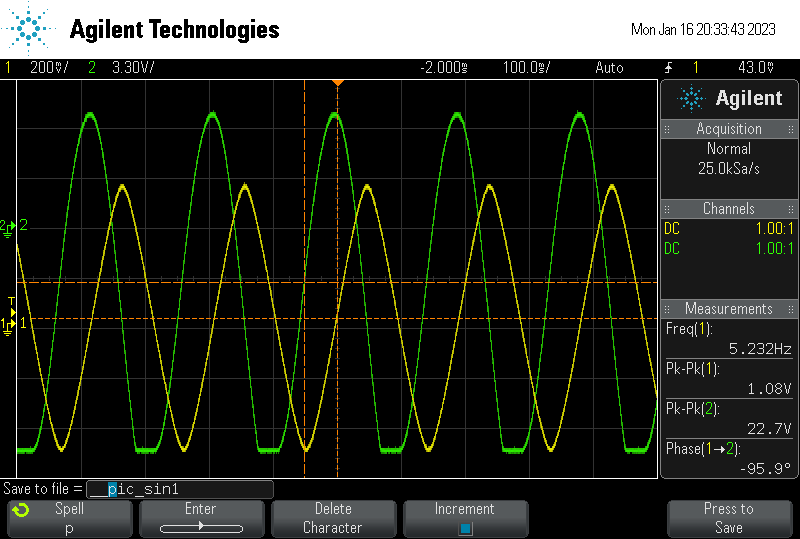
\includegraphics[width=0.6\textwidth]{python/data/__pic_sin1.png}
  \caption{Die Ausgabe des Ausgangssignals für den Integrator inklusive des Sinus-Eingangssignals. }
\label{fig:int_sin}
\end{figure}


\begin{figure}[H]
  \centering
  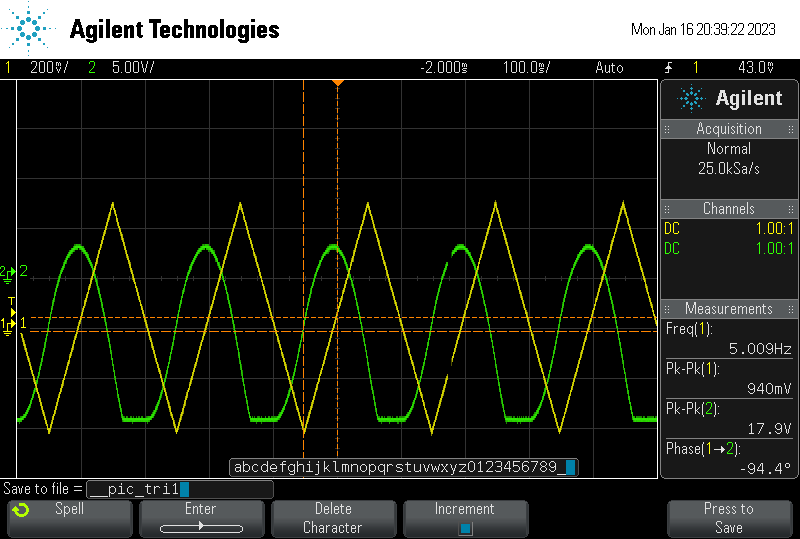
\includegraphics[width=0.6\textwidth]{python/data/__pic_tri1.png}
  \caption{Die Ausgabe des Ausgangssignals für den Integrator inklusive des Dreieck-Eingangssignals. }
\label{fig:int_dre}
\end{figure}


\begin{figure}[H]
  \centering
  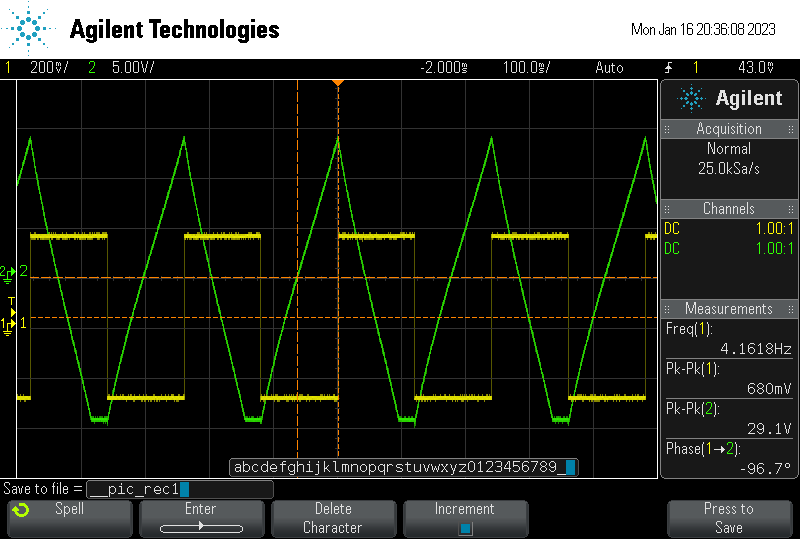
\includegraphics[width=0.6\textwidth]{python/data/__pic_rec1.png}
  \caption{Die Ausgabe des Ausgangssignals für den Integrator inklusive des Rechteck-Eingangssignals. }
\label{fig:int_recht}
\end{figure}


\subsection{Invertierter-Differenzierer}



\begin{figure}[H]
  \centering
  \includegraphics[width=0.6\textwidth]{build/plots/differenzierer.pdf}
  \caption{Die Messwerte des Verstärkungsfaktors des invertierten Differenzierers gegen die Frequenz aufgetragen}
\label{fig:diff1}
\end{figure}


\begin{figure}[H]
  \centering
  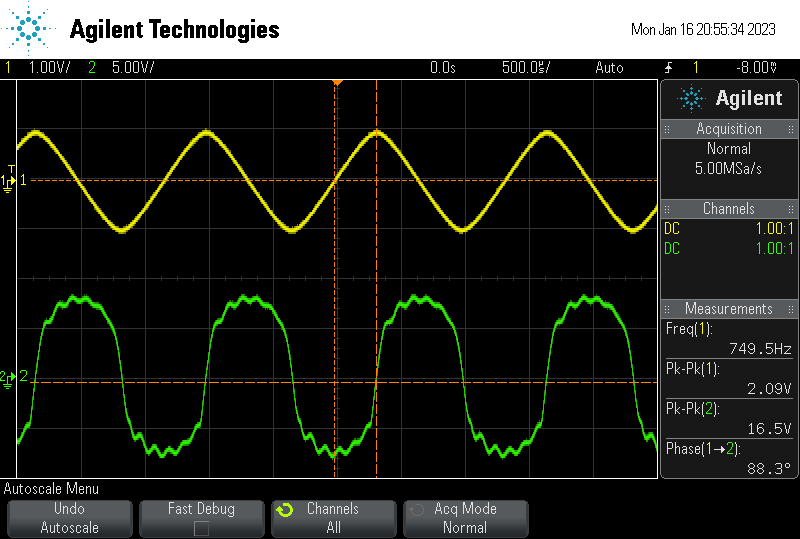
\includegraphics[width=0.6\textwidth]{python/data/__pic_sin2.png}
  \caption{Die Ausgabe des Ausgangssignals für den Differenzierer inklusive des Sinus-Eingangssignals. }
\label{fig:diff_sin}
\end{figure}


\begin{figure}[H]
  \centering
  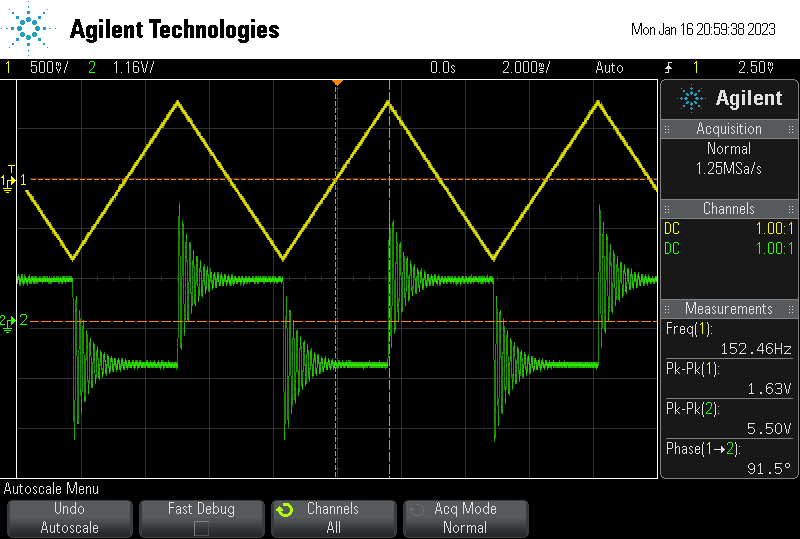
\includegraphics[width=0.6\textwidth]{python/data/__pic_tri2.png}
  \caption{Die Ausgabe des Ausgangssignals für den Differenzierer inklusive des Dreieck-Eingangssignals. }
\label{fig:diff_dre}
\end{figure}


\begin{figure}[H]
  \centering
  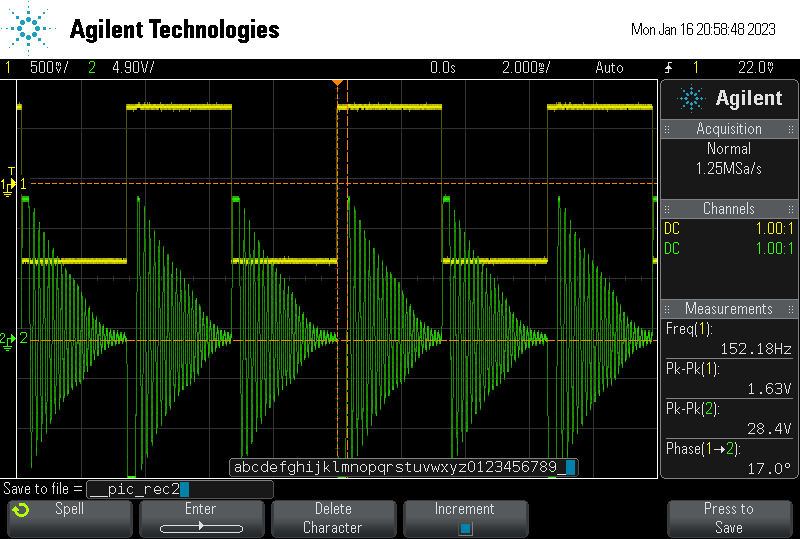
\includegraphics[width=0.6\textwidth]{python/data/__pic_rec2.png}
  \caption{Die Ausgabe des Ausgangssignals für den Differenzierer inklusive des Rechteck-Eingangssignals. }
\label{fig:diff_recht}
\end{figure}


\subsection{Nicht-invertierter-Schmitt-Trigger}



\subsection{Signalgenerator}






\begin{table}[ht]
\centering
\small
\caption{Messdaten zur Wien-Robinson-Brücke}
\label{tab:tab2}
\begin{tabular}{S [table-format=5.0] S [table-format=1.3]}
   \toprule
   {$\nu \mathbin{\scalebox{1.5} / } \si{\hertz}$} & $\text{Amplitude} \mathbin{\scalebox{1.5} / } \si{\volt}$\\
   \midrule
\end{tabular}
\end{table} 


%\begin{figure}
%    \centering
%    \includegraphics[width=0.6\textwidth]{build/plots/plot1.pdf}
%    \caption{Messdaten zur Wien-Robinson-Brücke}
%  \label{fig:plot1}
%\end{figure}
